%forwarding, patron de movimiento
\subsubsection{SMART}
SMART\cite{smart} es también una evolución de Spray-and-Wait, que incorpora el concepto de \emph{compañeros de viaje} de nodos --- es decir, nodos que frecuentemente se encuentran --- para mejorar la probabilidad de entrega sin propagar ni la historia de encuentros ni las probabilidades de entrega. Cada nodo propaga frecuentemente pequeños mensajes para declarar su presencia, con lo que cada nodos logra conocer con cuáles nodos comparte más frecuentemente. Con esta información un nodo envía $f_1-1$ copias del mensaje utilizando \emph{binary spray}, preguntando a los nodos que encuentra si son compañeros del destinatario. Al encontrar un compañero, éste a su vez envia $f_2-1$ mensajes a los compañeros del destinatario, esperando encontrarlo con mayor probabilidad que aquellos que no reconocen al destinatario como compañero. Los valores $f_1$ y $f_2$ son fijados en el protocolo, y deben adecuarse según el movimiento y topología donde se utilice.

\begin{figure}[h]
\centering
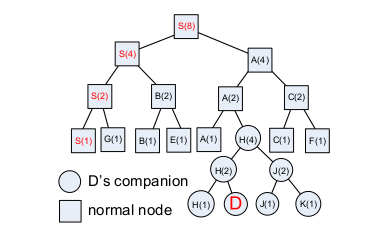
\includegraphics[width=200px]{smart.png}
\caption{Enrutamiento de SMART con $f_1 = 8$ y $f_2 = 4$ \cite{smart}}
\label{fig:smart}
\end{figure}

Esta estrategia es interesante al no requerir enviar información de encuentros de los otros nodos logrando incorporarla localmente. En simulaciones se observa que tiene una alta tasa de entrega (90\%), comparable a Epidemic, muy poco \emph{overhead} comparado a Epidemic, y una latencia menor que \cite{sandw}, aunque mayor que Epidemic, resultando ser una buena estrategia de incorporar inteligencia sin mucho procesamiento, a diferencia de Spray and Focus.